%!TEX program = xelatex
\documentclass[lang=cn,11pt,a4paper]{elegantpaper}

\title{数值积分的实现}
\author{第七小组: 刘阳 \quad 任浩辰 \\ 科目: 数值分析}
\date{\zhtoday}

\begin{document}

\maketitle

\section{实验目的}
通过编程实验,熟练掌握龙贝格公式及复合梯形公式,并比较二者的精度。

\section{实验步骤}
\begin{enumerate}
  \item 验证龙贝格公式的积分效果
  \item 验证龙贝格公式对复合梯形公式精度的提高
\end{enumerate}

\section{实验内容}
\subsection{复合梯形公式}
复合梯形公式的基础是梯形公式
\begin{equation}
  \int_{a}^{b} f(x)dx \approx \frac{b - a}{2} \lbrack f(a) + f(b) \rbrack
\end{equation}

为了提高求积精度,实际计算时可以将步长 $h$ 逐次分半
\begin{equation}
  \frac{h}{4} \lbrack f(x_k) + 2f(x_{k + \frac{1}{2}}) + f(x_{k + 1}) \rbrack
\end{equation}

注意,这里 $h = \frac{b - a}{2^{n-1}}$ 代表二分前的步长。将每个子区间上的积分值相加得
\begin{equation}
  T_n = \frac{h}{4} \sum_{k=0}^{n-1} \lbrack f(x_k) + f(x_{k+1}) \rbrack + \frac{h}{2} \sum_{k=0}^{n-1}f(x_{k+\frac{1}{2}})
\end{equation}

从而导出下列递推公式
\begin{equation} \label{T}
  T_{n+1} = \frac{1}{2} T_n + \frac{h}{2} \sum_{k=0}^{n-1} f(x_{k+\frac{1}{2}})
\end{equation}

其中
\begin{equation}
  T_1 = \frac{h}{2} \lbrack f(a) + f(b) \rbrack
\end{equation}

利用 $T_1$ 和 公式 (\ref{T}) ,我们可以递推地计算 $T_2, T_3, \cdots$

\subsection{龙贝格公式}
梯形法的算法虽然简单,但是精度低,收敛的速度缓慢,所以我们可以通过将精度较低的梯形法加工成高精度的方法,利用梯形公式的余项,并加以补偿我们可以得到
\begin{equation} \label{SCR}
  \begin{aligned}
    &S_n = T_{n+1} + \frac{1}{3}(T_{n+1} - T_n)
         = \frac{4}{3}T_{n+1} - \frac{1}{3}T_n \\
    &C_n = S_{n+1} + \frac{1}{15}(S_{n+1} - S_n)
         = \frac{16}{15}S_{n+1} - \frac{1}{15}S_n \\
    &R_n = C_{n+1} + \frac{1}{63}(C_{n+1} - C_n)
         = \frac{64}{63}C_{n+1} - \frac{1}{63}C_n
  \end{aligned}
\end{equation}

其中, $S_n$ 为辛甫生公式,$C_n$ 为柯特斯公式,$R_n$ 为龙贝格公式。

\begin{figure}[htbp]
  \centering
  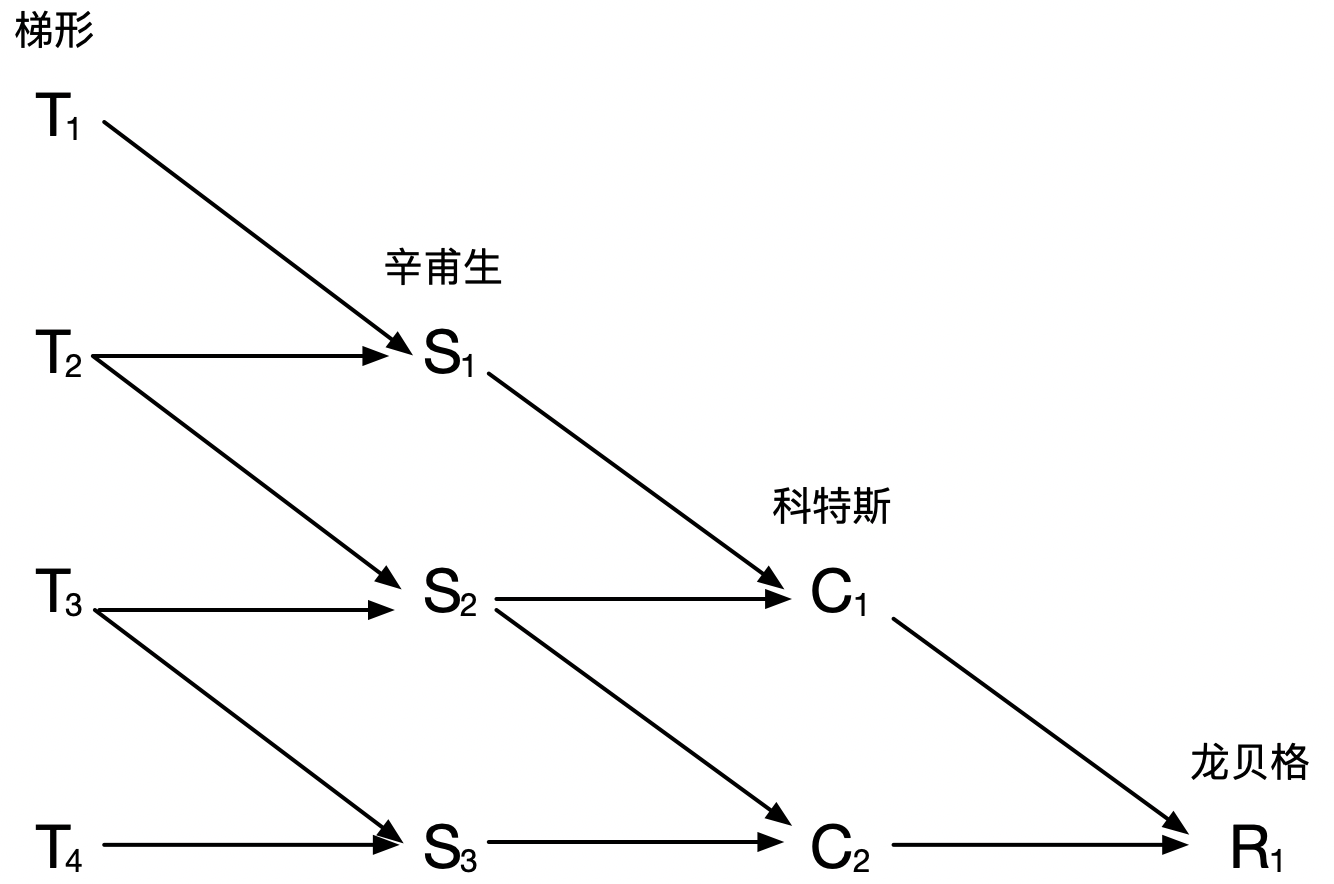
\includegraphics[width=0.5\textwidth]{image/TSCR.png}
\end{figure}

我们在步长二分的过程中运用公式(\ref{SCR})加工,就能将粗糙的积分值 $T_n$ 逐步加工成精度较高的龙贝格值 $R_n$,或者说,将收敛缓慢的梯形值序列 $T_n$ 加工成收敛迅速的龙贝格值序列 $R_n$。这种加速方法称龙贝格算法。

\section{实验过程及关键语句描写}
\subsection{验证龙贝格公式的积分效果}

这里所求的定积分是
$$
  I = \int_{0}^{1} \sqrt{2x - x^2}dx = \frac{\pi}{4} \approx 0.785398 
$$

\begin{lstlisting}[language=c++]
/// 被积函数 f(x)
double func(double x) {
  return sqrt(2 * x - x * x);
}
\end{lstlisting}

求二分点的函数值之和
$$
  \sum_{k=0}^{n-1} f(x_{k+\frac{1}{2}})
$$
\clearpage
\begin{lstlisting}[language=c++]
/// 二分点的函数值之和
double sum(double a, double b, double h) {
  double result = 0.0;
  
  double x = a;
  while (x < b) {
      result += func(x + h / 2);
      x += h;
  }

  return result;
}
\end{lstlisting}

使用龙贝格算法计算积分值,需要首先计算复合梯形公式的 $T_1, T_2, T_3, T_4$,进而计算出辛甫生公式的$S_1, S_2, S_3$ 和科特斯公式的 $C_1, C_2$,才能计算 $R_1$。
\begin{lstlisting}[language=c++]
#define REAL_VALUE 0.785398 // 真实值

double T[20];
double S[20];
double C[20];
double R[20];
int k = 4;

/// 龙贝格算法
void Romberg() {
  double a = 0.0;
  double b = 1.0;
  double h = b - a;
  T[1] = h / 2.0 * (func(a) + func(b));

  T[2] = T[1] / 2.0 + h / 2.0 * sum(a, b, h);
  h = h / 2.0;
  T[3] = T[2] / 2.0 + h / 2.0 * sum(a, b, h);
  h = h / 2.0;
  T[4] = T[3] / 2.0 + h / 2.0 * sum(a, b, h);
  h = h / 2.0;

  S[1] = T[2] + (T[2] - T[1]) / 3;
  S[2] = T[3] + (T[3] - T[2]) / 3;
  S[3] = T[4] + (T[4] - T[3]) / 3;

  C[1] = S[2] + (S[2] - S[1]) / 15;
  C[2] = S[3] + (S[3] - S[2]) / 15;

  R[1] = C[2] + (C[2] - C[1]) / 63;

  while (fabs(R[k - 3] - REAL_VALUE) >= 0.0000005) {
      k++;
      T[k] = T[k - 1] / 2.0 + h / 2.0 * sum(a, b, h);
      h = h / 2;
      S[k - 1] = T[k] + (T[k] - T[k - 1]) / 3;
      C[k - 2] = S[k - 1] + (S[k - 1] - S[k - 2]) / 15;
      R[k - 3] = C[k - 2] + (C[k - 2] - C[k - 3]) / 63;
  }
}
\end{lstlisting}

这里要求6位有效数字,即误差不大于 $5 \times 10^{-6}$。

\subsection{验证龙贝格公式对复合梯形公式精度的提高}
因为计算龙贝格公式需要复合梯形公式的数值,所以对比龙贝格公式和复合梯形公式,只要将储存在数组的数值取出即可。


\section{实验结果}
\subsection{验证龙贝格公式的积分效果}
通过调用龙贝格算法计算积分值并计算与真实值的误差。
\begin{figure}[htbp]
  \centering
  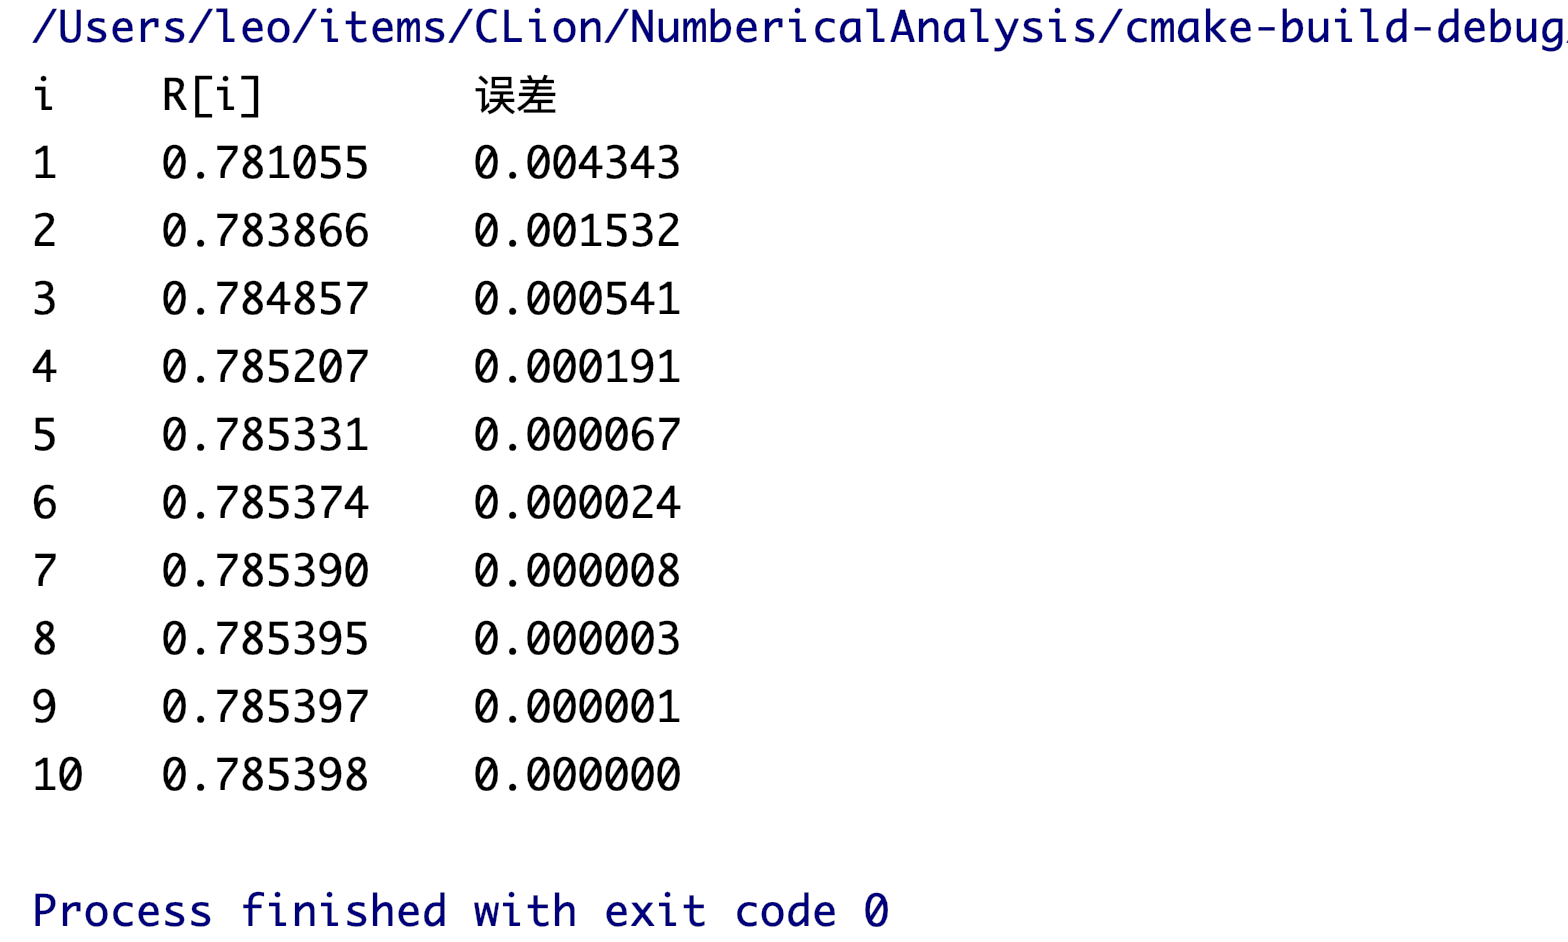
\includegraphics[width=0.5\textwidth]{image/Romberg_1.png}
\end{figure}

可以看出龙贝格公式的精度还是很高的,在使用一次龙贝格公式是精度就已经达到 2 位有效数字了。
并且精度上升得很快,再递推调用数次龙贝格公式后得出的数值已经很接近真实值了。

\subsection{验证龙贝格公式对复合梯形公式精度的提高}
将储存在数组中的复合梯形公式、辛甫生公式、科特斯公式以及龙贝格公式的计算数值打印成下三角数表,比较它们的精度。
\clearpage

\begin{figure}[htbp]
  \centering
  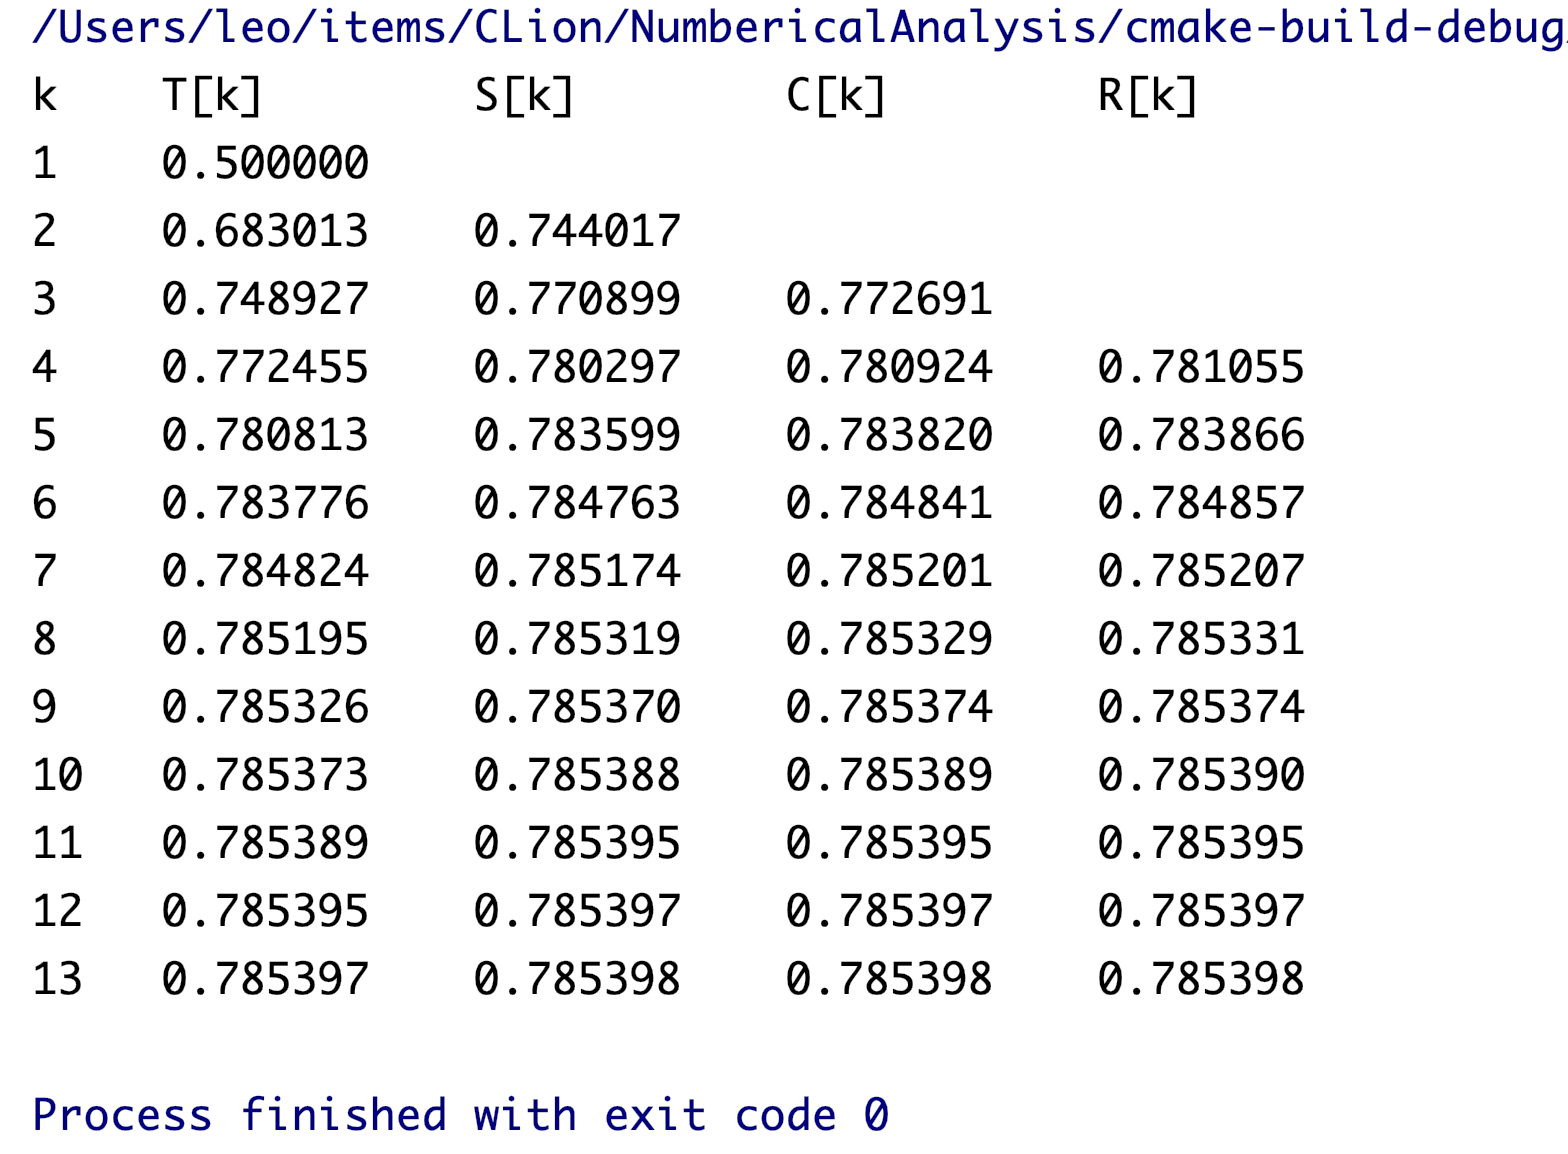
\includegraphics[width=0.5\textwidth]{image/Romberg_2.png}
\end{figure}

进一步,对比复合梯形公式和龙贝格公式对于真实值的误差。
\begin{figure}[htbp]
  \centering
  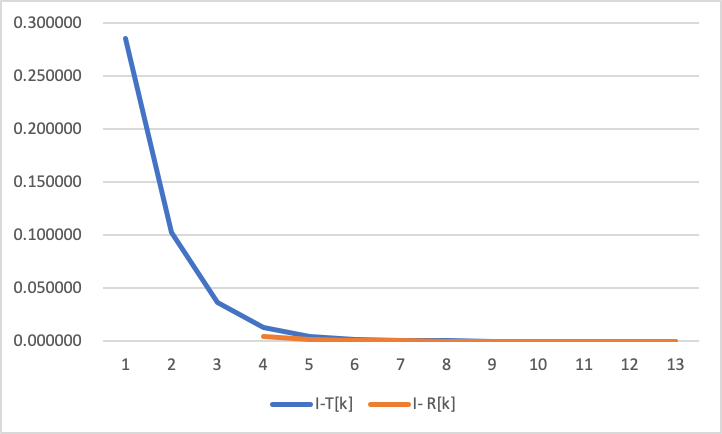
\includegraphics[width=0.5\textwidth]{image/T_R.png}
\end{figure}

我们可以发现龙贝格公式能够很好的加速数值积分收敛到积分真实值,并且龙贝格公式的收敛速度大于复合梯形公式的收敛速度。
所以使用龙贝格公式能够很好的计算数值积分,获得较高精度的数值。


\section{实验体会}
\begin{enumerate}
  \item 龙贝格算法比较简单,只需要计算需要首先计算复合梯形公式的 $T_1, T_2, T_3, T_4$、辛甫生公式的$S_1, S_2, S_3$、科特斯公式的 $C_1, C_2$和龙贝格公式的$R_1$,
  就能够递推地使用龙贝格算法计算数值积分,直到精度符合要求。
  \item 本次实验通过使用 C++ 编程实现了龙贝格算法,发现龙贝格公式能够在有限的计算次数快速收敛到积分的真实值,
  计算速度快而且精度高。
  \item 龙贝格算法通过递推地补偿复合梯形公式的余项误差,使得误差较小。所以说在有限的等距的函数值时,通过使用龙贝格公式能够获得精度最高的积分值。
\end{enumerate}

\end{document}
